% Project report — Formal Languages (SI2002 / ST0270 / CM0081)
% Compile with:  pdflatex Informe.tex   (twice)   or   tectonic -X compile Informe.tex
% Figures are in figuras/; the grammars are in docs/.
\documentclass[11pt,letterpaper]{article}

\usepackage[utf8]{inputenc}
\usepackage[T1]{fontenc}
\usepackage{lmodern}
\usepackage[english]{babel}
\usepackage{amsmath,amssymb}
\usepackage{booktabs}
\usepackage{tabularx}
\usepackage{longtable}
\usepackage{array}
\usepackage{graphicx}
\usepackage{xcolor}
\usepackage[margin=2.4cm]{geometry}
\usepackage{listings}
\usepackage{float}
\usepackage{caption}
\usepackage{enumitem}
\usepackage{fancyhdr}
\usepackage[hidelinks]{hyperref}

\definecolor{azul}{HTML}{1F3864}
\definecolor{grisclaro}{HTML}{F2F2F2}

\lstdefinestyle{codigo}{
  basicstyle=\ttfamily\footnotesize,
  backgroundcolor=\color{grisclaro},
  frame=single, rulecolor=\color{gray!50},
  breaklines=true, columns=fullflexible,
  keepspaces=true, showstringspaces=false,
  aboveskip=6pt, belowskip=6pt
}
\lstdefinestyle{consola}{
  basicstyle=\ttfamily\footnotesize,
  backgroundcolor=\color{grisclaro},
  frame=single, rulecolor=\color{gray!50},
  breaklines=true, columns=fullflexible,
  keepspaces=true, showstringspaces=false,
  aboveskip=6pt, belowskip=6pt
}

\pagestyle{fancy}
\fancyhf{}
\fancyhead[L]{\footnotesize Formal Languages --- Project report}
\fancyhead[R]{\footnotesize SI2002 / ST0270 / CM0081}
\fancyfoot[C]{\footnotesize \thepage}
\renewcommand{\headrulewidth}{0.4pt}

\captionsetup{font=small,labelfont=bf}
\setlength{\parskip}{4pt}
\setlength{\parindent}{0pt}

\newcommand{\nt}[1]{\texttt{#1}}
\newcommand{\attr}[1]{\texttt{#1}}

\title{\vspace{-1.2cm}\textbf{\color{azul}Project Report}\\[4pt]
\large FIRST and FOLLOW sets, LL(1) and SLR(1) parsers,\\
\large and evaluation of a syntax-directed definition}
\author{Juan David Giraldo Regino \and Camilo Andrés Rodríguez Agudelo \and Daniel Rojas Grajales}
\date{Formal Languages --- SI2002 / ST0270 Formal Languages and Compilers / CM0081\\ November 2026}

\begin{document}

\begin{titlepage}
\centering
\vspace*{2.4cm}
{\color{azul}\rule{\textwidth}{1.2pt}}\\[14pt]
{\LARGE\bfseries\color{azul} Project Report}\\[10pt]
{\large FIRST and FOLLOW sets, LL(1) and SLR(1) parsers,\\[2pt]
and evaluation of a syntax-directed definition}\\[12pt]
{\color{azul}\rule{\textwidth}{1.2pt}}\\[2.2cm]

\begin{tabular}{c}
\large Juan David Giraldo Regino\\
\large Camilo Andrés Rodríguez Agudelo\\
\large Daniel Rojas Grajales
\end{tabular}

\vspace{1.6cm}
Formal Languages --- SI2002 / ST0270 Formal Languages and Compilers /\\
CM0081 Formal Languages and Automata

\vspace{1.4cm}
November 2026

\vfill
\begin{minipage}{0.86\textwidth}
\centering\small
Implementation: Python 3, standard library only (no parser generators, no parsing libraries).\\
Repository: \url{https://github.com/ArrozConPollo7/lenguajes-formales-parser}
\end{minipage}
\end{titlepage}

\tableofcontents
\newpage

\section{Introduction}

This report documents the four items of the project: the computation of the FIRST and FOLLOW
sets, the LL(1) and SLR(1) parsers, a syntax-directed definition (SDD) evaluated with the
dependency-graph method, and the problems found while implementing the previous three. The
implementation is written in Python 3 using only the standard library: no parser generator and no
library that computes FIRST/FOLLOW sets, LR automata or parsing tables is used. The input grammar
is never transformed: it is tested exactly as it is written, so a left-recursive grammar is
reported as not LL(1) instead of being rewritten.

Every algorithm follows the book (Aho, Lam, Sethi and Ullman, \emph{Compilers: Principles,
Techniques, and Tools}, 2nd edition). Table~\ref{tab:partes} says, for each part, the section of
the book and the function that implements it.

\begin{table}[H]
\centering
\footnotesize
\caption{Book section, algorithm or figure followed for each part, and the function that implements it.}
\label{tab:partes}
\begin{tabularx}{\textwidth}{@{}>{\raggedright\arraybackslash}X >{\raggedright\arraybackslash}p{3.6cm} >{\raggedright\arraybackslash}p{2.5cm} >{\raggedright\arraybackslash}p{4.6cm}@{}}
\toprule
\textbf{Part} & \textbf{Book} & \textbf{File} & \textbf{Functions}\\
\midrule
FIRST and FOLLOW by fixed point & 4.4.2, pp. 220--222 & \nt{first\_follow.py} & \nt{first\_de\_simbolos}, \nt{follow}\\
LL(1) test and table $M[A,a]$ & 4.4.3, Algorithm 4.31, p. 224 & \nt{ll1.py} & \nt{construir\_tabla}, \nt{es\_ll1}\\
Predictive parser with a stack & 4.4.4, Algorithm 4.34, Fig. 4.20, pp. 226--227 & \nt{ll1.py} & \nt{parsear\_ll1}\\
Shift-reduce parsing and conflicts & 4.5.4 & --- & background only\\
LR(0) items, CLOSURE, GOTO, canonical collection & 4.6.2, Figs. 4.32--4.33, pp. 242--246 & \nt{slr1.py} & \nt{cerradura}, \nt{goto}, \nt{automata\_lr0}\\
ACTION/GOTO of SLR(1) from FOLLOW & 4.6.4, Algorithm 4.46, pp. 253--254 & \nt{slr1.py} & \nt{construir\_tablas}, \nt{es\_slr1}\\
LR parsing algorithm & 4.6.3, Algorithm 4.44, Fig. 4.36, pp. 250--251 & \nt{slr1.py} & \nt{parsear\_lr}\\
Synthesized/inherited attributes, annotated tree & 5.1.1--5.1.2, pp. 304--305 & \nt{sdd.py} & \nt{TABLA\_ATRIBUTOS}, \nt{texto\_arbol}\\
Dependency graph and topological order & 5.2.1, pp. 310--311; 5.2.2, p. 312 & \nt{sdd.py} & \nt{grafo\_dependencias}, \nt{orden\_topologico}\\
S-attributed and L-attributed definitions & 5.2.3, pp. 312--313; 5.2.4, pp. 313--314 & \nt{sdd.py} & classification (Sec. 4.5)\\
\bottomrule
\end{tabularx}
\end{table}

\subsection{Data structures}

\begin{itemize}[leftmargin=1.1em,itemsep=2pt]
\item \textbf{Grammar}: a dictionary \nt{\{nonterminal: [body, ...]\}} where each body is a
\textbf{tuple of symbols}. The empty body is the empty tuple, never the character \nt{e}: FIRST of
a string, the item $A \to \cdot$ and the reduction of an empty body then need no special case, and
\nt{e} is written back only when printing.
\item \textbf{Numbered production list}: \nt{[(head, body), ...]} in input order. The index in this
list is the identity of a production: an LR(0) item is \nt{(production\_index, dot\_position)} and a
semantic rule is attached to that same index. Without this shared identity a rule could be attached
to the wrong production.
\item \textbf{Parse tree}: one class \nt{Nodo} (symbol, production index, children, attribute values)
used by both parsers, so the same string produces the same tree with LL(1) and with SLR(1) and the
SDD does not care which parser built it.
\item \textbf{LR(0) item sets}: \nt{frozenset} of items; the canonical collection is a list of sets
and the transitions a dictionary \nt{\{(state, symbol): state\}}.
\item \textbf{Parsing tables}: dictionaries keyed by a state and a terminal for ACTION and by a
state and a nonterminal for GOTO, so no fixed alphabet is assumed.
\item \textbf{SDD}: data, not code. For each production there is a list of rules and each rule is a
dictionary with the attribute it defines, the attributes it uses, and the function that computes
it. The evaluator knows nothing about the particular SDD.
\end{itemize}

\section{Item 1: FIRST and FOLLOW}

FIRST is computed for every grammar symbol and then extended to strings (Section 4.4.2). The
function iterates until no set changes: FIRST(X) is enlarged with FIRST of the body of every
production $X \to Y_1\cdots Y_k$, and $\varepsilon$ is added to FIRST(X) only when $X \to
\varepsilon$ or when every symbol of the body can derive $\varepsilon$. FOLLOW(A) starts with \$ when
$A$ is the start symbol and is enlarged by three rules: the symbols after $A$ in a body contribute
their FIRST set without $\varepsilon$; the symbols that can follow $A$ at the end of a body
contribute FOLLOW of the head; and if $A$ is at the end of the body then FOLLOW(head) $\subseteq$
FOLLOW($A$). The fixed point is necessary because $\varepsilon$-chains propagate both sets: a single
sweep in input order can leave a set incomplete.

The program prints the sets with \nt{-{}-sets}, one line per nonterminal in alphabetical order, with
the terminals in ASCII order followed by \nt{e} and then \nt{\$}.

\subsection{Grammar of our own (Items 1 and 2)}

To exercise the parsers we wrote grammar $G_1$, a small language of \emph{blocks}: a block is a
sequence of items separated by \nt{;}, and an item is either the letter \nt{x} or a bracketed block.
It is not one of the examples of the assignment, it is left recursive (so it cannot be LL(1) unless
it is transformed, which is forbidden), and it is SLR(1), which is exactly the combination we want
to show.

\begin{lstlisting}[style=codigo]
3
S -> L
L -> L;E E
E -> x [L]
\end{lstlisting}

Production 1 ($L \to L\,;E$) makes $L$ left recursive; that is what breaks the LL(1) test and what
the SLR(1) automaton handles by shifting the \nt{;}.

FIRST and FOLLOW computed by the program (\nt{-{}-sets}). After the sets the program continues
with the applicable case, which is why the last line says that the grammar is SLR(1):

\begin{lstlisting}[style=consola]
$ python3 main.py --sets < docs/gramatica_ejemplo.txt
First(E) = {[, x}
Follow(E) = {;, ], $}
First(L) = {[, x}
Follow(L) = {;, ], $}
First(S) = {[, x}
Follow(S) = {$}
Grammar is SLR(1).
\end{lstlisting}

\nt{FOLLOW(E) = \{ ;, ], \$ \}} is worth tracing by hand: $S \to L$ gives FOLLOW(L) $\supseteq$
\{\$\}, and since $L$ is at the end of that body also FOLLOW(L) $\subseteq$ FOLLOW(S); in $L \to
L\,;E$ the symbol \nt{;} precedes $E$ and $E$ ends the body, so FOLLOW(E) $\supseteq$ FOLLOW(L); and
in $E \to [\,L\,]$ the symbol after $L$ is \nt{]}, which enters FOLLOW(L) and from there FOLLOW(E).
That is why the closing bracket ends up in FOLLOW(E) even though $E$ never appears before a
\nt{]}.

\section{Item 2: LL(1) and SLR(1) parsers}

\subsection{The grammar is not LL(1)}

The predictive table is built with the two rules of Section 4.4.3: for each production $A \to
\alpha$, add it to $M[A,a]$ for every $a \in \mathrm{FIRST}(\alpha)$, and if $\varepsilon \in
\mathrm{FIRST}(\alpha)$ also for every $a \in \mathrm{FOLLOW}(A)$. The grammar is LL(1) if and only
if no cell receives two different productions. For $G_1$ the program reports the conflicting cells
of Table~\ref{tab:conflictos}.

\begin{table}[H]
\centering
\small
\caption{Conflicting cells of the predictive table of $G_1$.}
\label{tab:conflictos}
\begin{tabularx}{\textwidth}{@{}l l >{\raggedright\arraybackslash}X@{}}
\toprule
\textbf{Cell} & \textbf{Productions that collide} & \textbf{Why}\\
\midrule
$M[L,\nt{x}]$ & 1: $L \to L\,;E$ \newline 2: $L \to E$ &
FIRST($L\,;E$) = FIRST($L$) = \{\nt{[}, \nt{x}\}: the left recursion makes both alternatives start
with the same terminals, so no lookahead of one symbol can choose between them.\\
$M[L,\nt{]}]$ & 1: $L \to L\,;E$ \newline 2: $L \to E$ & Same reason.\\
\bottomrule
\end{tabularx}
\end{table}

This is the expected consequence of not transforming the grammar: removing the left recursion would
produce an equivalent grammar that is LL(1), but the assignment forbids it and the left recursion
itself is the evidence that the grammar, as written, is not LL(1).

\subsection{The grammar is SLR(1)}

The grammar is augmented with $S' \to S$ (Section 4.6.2) and the canonical collection of LR(0) item
sets is built with CLOSURE and GOTO. The augmented production is appended \emph{after} the original
ones so the original indices --- and therefore the items and the semantic rules --- keep their
numbering. The program obtains 10 states (Table~\ref{tab:estados}).

\begin{table}[H]
\centering
\small
\caption{LR(0) item sets of $G_1$ (10 states), as built by the program.}
\label{tab:estados}
\begin{tabularx}{\textwidth}{@{}l >{\raggedright\arraybackslash}X@{}}
\toprule
\textbf{State} & \textbf{LR(0) items}\\
\midrule
I0 & S $\to$ .L; L $\to$ .L;E; L $\to$ .E; E $\to$ .x; E $\to$ .[L]; S' $\to$ .S \\
I1 & L $\to$ E. \\
I2 & S $\to$ L.; L $\to$ L.;E \\
I3 & S' $\to$ S. \\
I4 & L $\to$ .L;E; L $\to$ .E; E $\to$ .x; E $\to$ .[L]; E $\to$ [.L] \\
I5 & E $\to$ x. \\
I6 & L $\to$ L;.E; E $\to$ .x; E $\to$ .[L] \\
I7 & L $\to$ L.;E; E $\to$ [L.] \\
I8 & L $\to$ L;E. \\
I9 & E $\to$ [L]. \\
\bottomrule
\end{tabularx}
\end{table}

The ACTION table uses shift for terminals after the dot, reduce $A \to \alpha$ in every terminal of
FOLLOW($A$) when the dot reached the end, and accept only for $S' \to S$ with \nt{\$}; GOTO is
filled only for nonterminals. Tables~\ref{tab:action} and~\ref{tab:goto} are the tables produced by
the program ($\mathrm{s}j$ = shift to state $j$, $\mathrm{r}i$ = reduce production $i$, acc =
accept; the empty cell is an error entry).

\begin{table}[H]
\centering
\small
\caption{ACTION table of $G_1$.}
\label{tab:action}
\begin{tabular}{@{}l ccccc@{}}
\toprule
\textbf{State} & \nt{x} & \nt{;} & \nt{[} & \nt{]} & \nt{\$}\\
\midrule
I0 & s5 & & s4 & & \\
I1 & & r2 & & r2 & r2\\
I2 & & s6 & & & r0\\
I3 & & & & & acc\\
I4 & s5 & & s4 & & \\
I5 & & r3 & & r3 & r3\\
I6 & s5 & & s4 & & \\
I7 & & s6 & & s9 & \\
I8 & & r1 & & r1 & r1\\
I9 & & r4 & & r4 & r4\\
\bottomrule
\end{tabular}
\end{table}

\begin{table}[H]
\centering
\small
\caption{GOTO table of $G_1$.}
\label{tab:goto}
\begin{tabular}{@{}l ccc@{}}
\toprule
\textbf{State} & \nt{S} & \nt{L} & \nt{E}\\
\midrule
I0 & 3 & 2 & 1\\
I1 & & & \\
I2 & & & \\
I3 & & & \\
I4 & & 7 & 1\\
I5 & & & \\
I6 & & & 8\\
I7 & & & \\
I8 & & & \\
I9 & & & \\
\bottomrule
\end{tabular}
\end{table}

There is no conflicting cell (the program reports an empty list of conflicts), so the grammar is
SLR(1). Some states explain why. In I2 the items are $S \to L\cdot$ and $L \to L\cdot;E$: following
$L$ the parser shifts \nt{;} and reduces $S \to L$ only on \nt{\$}, because FOLLOW(S) = \{\$\}. In I7
the items are $L \to L\cdot;E$ and $E \to [L\cdot\,]$: the decision is taken with the terminal of the
input, \nt{;} or \nt{]}, which are different terminals, so there is no conflict either. In a state
where a reduce and a shift compete for the \emph{same} terminal the FOLLOW set is what decides, and
here it never overlaps.

\subsection{One string parsed step by step}

The string \nt{[x;x];x} is generated by $G_1$: a block that contains \nt{x;x}, then \nt{;x}. The
Table~\ref{tab:traza} is the trace registered by the LR parser (Section 4.6.3); the stack holds
states and $\mid$ marks how much of the input has been consumed.

\begin{longtable}{@{}lll@{}}
\caption{Trace of the LR parser on \nt{[x;x];x}.}\label{tab:traza}\\
\toprule
\textbf{Stack} & \textbf{Input} & \textbf{Action}\\
\midrule
\endfirsthead
\toprule
\textbf{Stack} & \textbf{Input} & \textbf{Action}\\
\midrule
\endhead
\bottomrule
\endfoot
\scriptsize
0 & $\mid$ [x;x];x\$ & shift 4 \\
0 4 & [ $\mid$ x;x];x\$ & shift 5 \\
0 4 5 & [x $\mid$ ;x];x\$ & reduce E $\to$ x \\
0 4 1 & [E $\mid$ ;x];x\$ & reduce L $\to$ E \\
0 4 7 & [L $\mid$ ;x];x\$ & shift 6 \\
0 4 7 6 & [L; $\mid$ x];x\$ & shift 5 \\
0 4 7 6 5 & [L;x $\mid$ ];x\$ & reduce E $\to$ x \\
0 4 7 6 8 & [L;E $\mid$ ];x\$ & reduce L $\to$ L;E \\
0 4 7 & [L $\mid$ ];x\$ & shift 9 \\
0 4 7 9 & [L] $\mid$ ;x\$ & reduce E $\to$ [L] \\
0 1 & E $\mid$ ;x\$ & reduce L $\to$ E \\
0 2 & L $\mid$ ;x\$ & shift 6 \\
0 2 6 & L; $\mid$ x\$ & shift 5 \\
0 2 6 5 & L;x $\mid$ \$ & reduce E $\to$ x \\
0 2 6 8 & L;E $\mid$ \$ & reduce L $\to$ L;E \\
0 2 & L $\mid$ \$ & reduce S $\to$ L \\
0 3 & S $\mid$ \$ & accept \\
\end{longtable}

The parser accepts. The tree it built is the following (preorder, with the production applied at
each node):

\begin{lstlisting}[style=codigo]
S   (S -> L)
  L   (L -> L;E)
    L   (L -> E)
      E   (E -> [L])
        [
        L   (L -> L;E)
          L   (L -> E)
            E   (E -> x)
              x
          ;
          E   (E -> x)
            x
        ]
    ;
    E   (E -> x)
      x
\end{lstlisting}

\section{Item 3: the syntax-directed definition}

\subsection{The grammar}

Grammar $G_2$ generates decimal numerals --- a nonempty sequence of digits, leading zeros allowed
--- and the empty numeral; the SDD computes the integer value of the numeral. It satisfies the three
conditions of Step 1: it follows the input conventions of Section 2.2 and is both LL(1) and SLR(1)
(checked by the program), it has three nonterminals, thirteen productions and the recursive
nonterminal \nt{N}, and it is not a grammar of the book or of the assignment: instead of the usual
desk-calculator examples, the value of a numeral is computed from the \emph{position} of each digit,
which needs an inherited attribute because the position is counted from the right.

On condition G3, the closest idea in the book is Exercise~5.2.4, which asks the reader to design an
L-attributed SDD for binary numerals with a decimal point; that is an exercise without a solution in
the text, and our grammar and our SDD are both different: the grammar is decimal, allows
$\varepsilon$ and leading zeros and has no fractional part, and the SDD computes not only the value
but also the length of the numeral, from which the exponent of each digit is derived --- which is
precisely the dependency $N.len \to N.e$ that a simpler scheme for the same idea does not have.

\begin{lstlisting}[style=codigo]
3
S -> N
N -> DN e
D -> 0 1 2 3 4 5 6 7 8 9
\end{lstlisting}

The grammar generates $\{0,\dots,9\}^{*}$ (including the empty numeral), and both parsers accept
exactly that language; the test suite checks that they build the same tree.

\subsection{Attributes}

\begin{table}[H]
\centering
\small
\caption{Attributes of the SDD of $G_2$.}
\label{tab:atributos}
\begin{tabularx}{\textwidth}{@{}c c l l >{\raggedright\arraybackslash}X@{}}
\toprule
\textbf{Symbol} & \textbf{Attribute} & \textbf{Kind} & \textbf{Type} & \textbf{Meaning}\\
\midrule
S & \attr{v} & synthesized & integer & value of the numeral represented by the string (main attribute)\\
N & \attr{len} & synthesized & integer & number of digits in the subtree of \nt{N}\\
N & \attr{e} & inherited & integer & exponent (power of ten) of the first digit of \nt{N}\\
N & \attr{v} & synthesized & integer & value of the numeral represented by \nt{N}\\
D & \attr{e} & inherited & integer & exponent (power of ten) of that digit\\
D & \attr{v} & synthesized & integer & numeric value of the digit\\
digit & \attr{lexval} & synthesized & character & the character of the digit (provided by the scanner; here it is the character itself)\\
\bottomrule
\end{tabularx}
\end{table}

Terminals have only \attr{lexval}, the character itself, which the scanner provides; that is why the
program does not need a real scanner. The start symbol \nt{S} has no inherited attribute, as
required, and the test suite verifies it.

\subsection{Semantic rules}

\begin{table}[H]
\centering
\small
\caption{Semantic rules of the SDD (format of Figure 5.1).}
\label{tab:reglas}
\begin{tabularx}{\textwidth}{@{}l >{\raggedright\arraybackslash}X@{}}
\toprule
\textbf{Production} & \textbf{Semantic rules}\\
\midrule
$S \to N$ & $N.e = N.len - 1$;\quad $S.v = N.v$\\
$N \to D\,N_1$ & $D.e = N.e$;\quad $N_1.e = N.e - 1$;\quad $N.len = N_1.len + 1$;\quad
$N.v = D.v \cdot 10^{D.e} + N_1.v$\\
$N \to \varepsilon$ & $N.len = 0$;\quad $N.v = 0$\\
$D \to d$ \ (any digit) & $D.v = $ integer value of $d.lexval$\\
\bottomrule
\end{tabularx}
\end{table}

Every rule defines either a synthesized attribute of the head or an inherited attribute of a symbol
of the body, using only attributes of the same production; for each production every synthesized
attribute of the head and every inherited attribute of a nonterminal of the body is defined
exactly once (the test suite checks this automatically over the rule table).

\subsection{Step 3: one string worked by hand}

Take the string \nt{1207} (four terminals). Its annotated parse tree is shown in
Figure~\ref{fig:arbol}: every node shows the label used by the program (symbol and preorder
position) and the value of each of its attributes.

\begin{figure}[H]
\centering
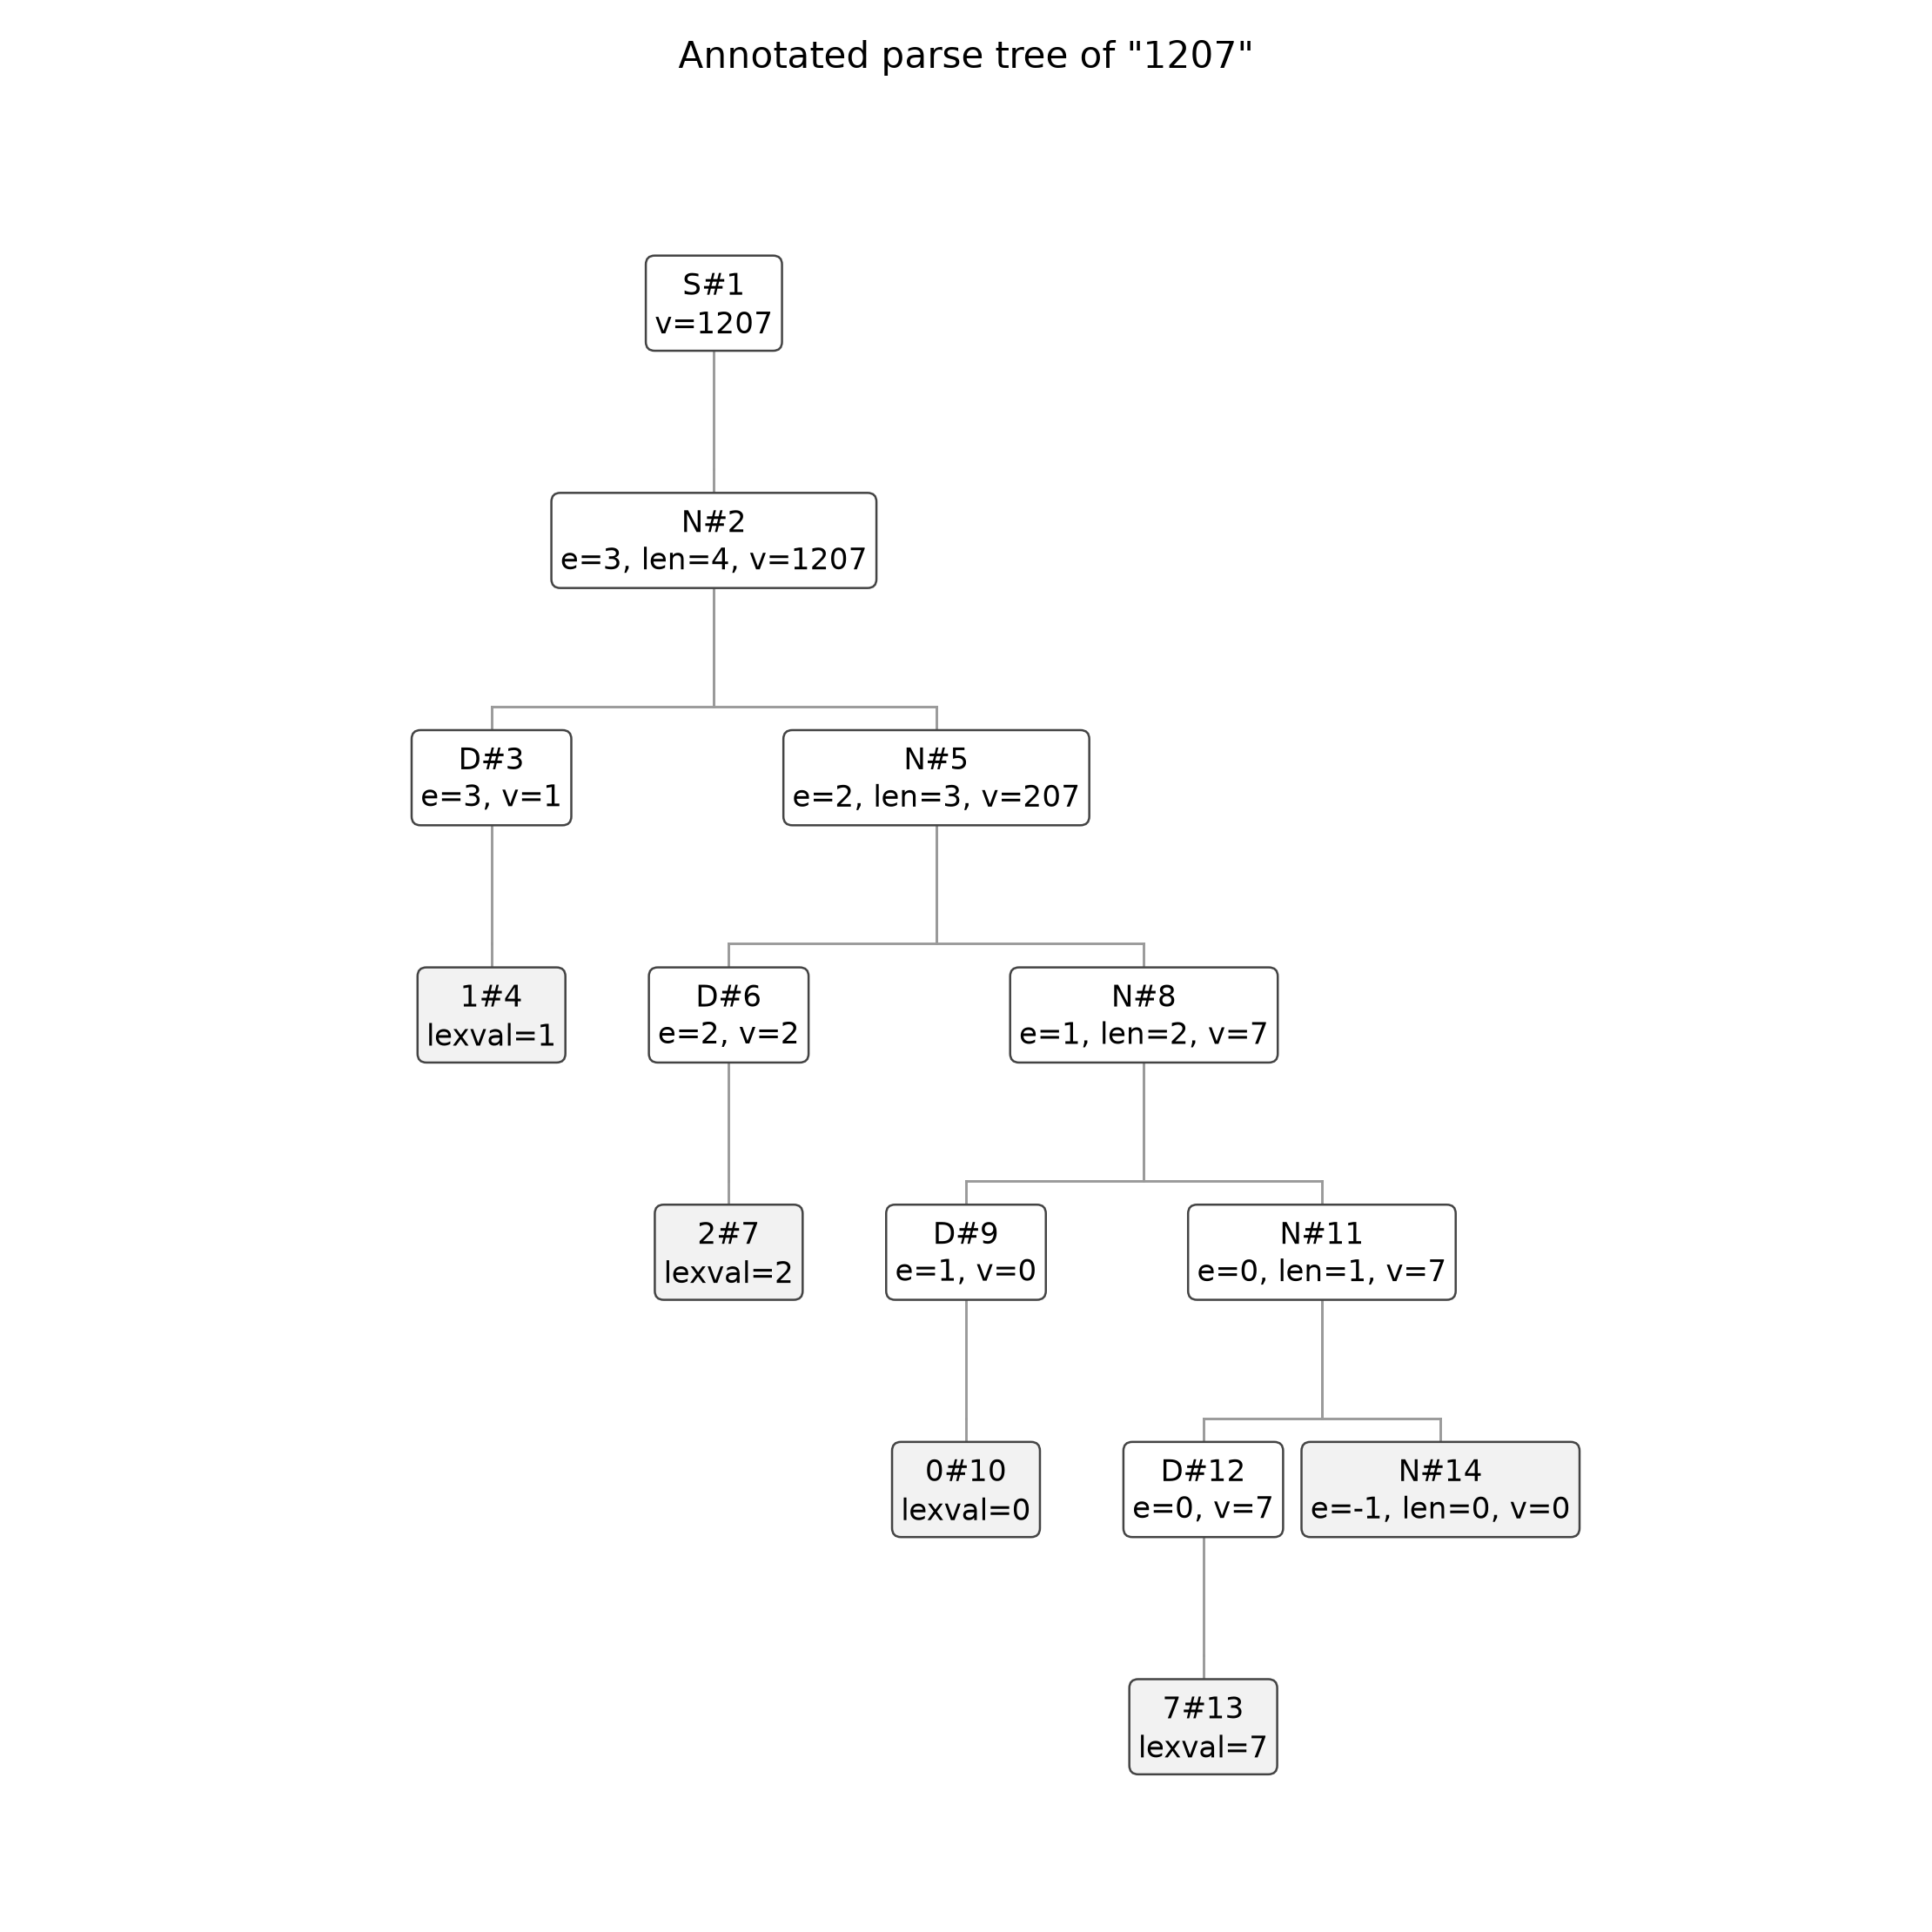
\includegraphics[width=0.97\textwidth]{figuras/arbol.png}
\caption{Annotated parse tree of \nt{1207}: $e$ is the exponent (power of ten) of the digit,
\attr{len} the number of digits of the subtree and \attr{v} the value it represents.}
\label{fig:arbol}
\end{figure}

The values agree with the definition: the rightmost digit 7 sits on $10^0$, the 0 on $10^1$, the 2 on
$10^2$ and the 1 on $10^3$, so $1\cdot1000 + 2\cdot100 + 0\cdot10 + 7 = 1207$, which is the value
printed for \attr{S.v}.

The dependency graph instantiates every rule of every production used in the tree: one vertex for
each attribute of each node and one edge from each attribute that is used to the attribute that is
defined (Section 5.2.1). The graph of this tree has 28 vertices and no cycle
(Figure~\ref{fig:grafo}).

\begin{figure}[H]
\centering
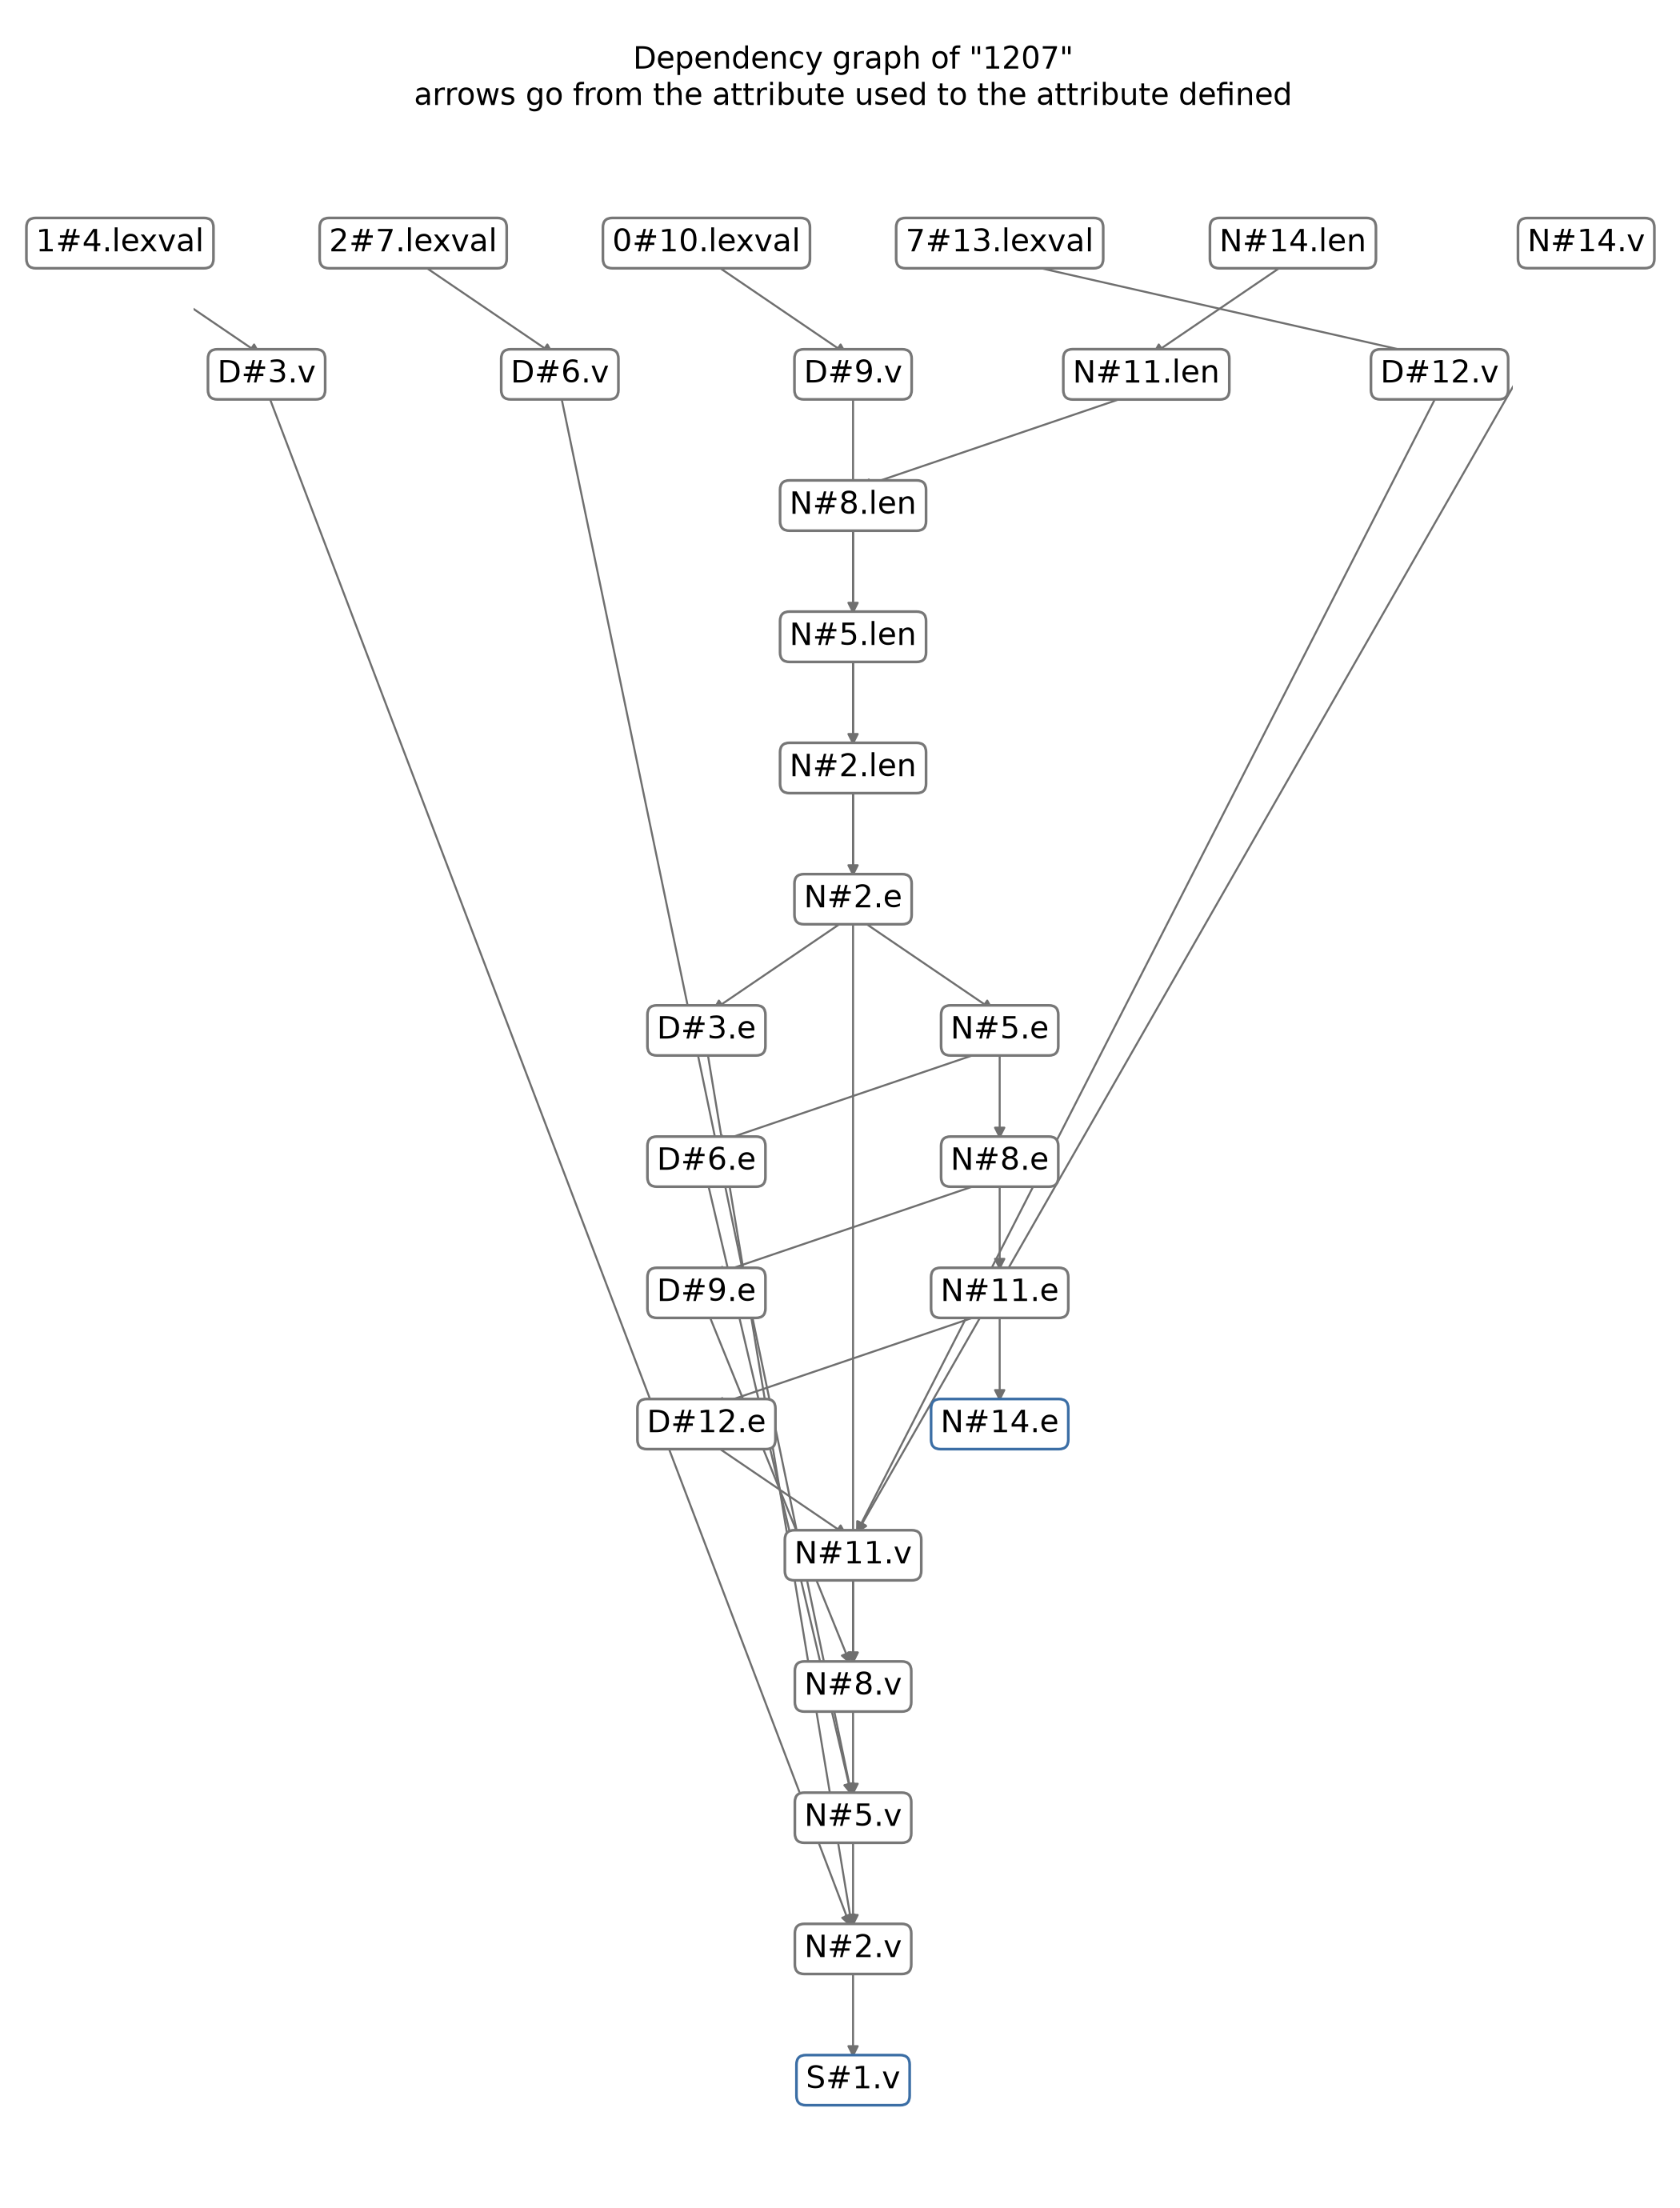
\includegraphics[width=0.72\textwidth]{figuras/grafo.png}
\caption{Dependency graph of the tree of \nt{1207}, drawn in layers: every arrow goes from an
attribute to one in a lower layer, so the layers are a topological order. Vertex \attr{N\#2.e}
depends on \attr{N\#2.len}: that edge goes up inside one node and is the reason a single pass
cannot evaluate the tree (Section 4.5).}
\label{fig:grafo}
\end{figure}

One valid evaluation order --- the one the program computes and prints --- is
Table~\ref{tab:orden}. It is a topological order: each attribute appears after all the attributes
it depends on.

\begin{table}[H]
\centering
\small
\caption{Evaluation order computed by the program for \nt{1207} (28 attributes).}
\label{tab:orden}
\begin{tabular}{@{}r l r l r l@{}}
\toprule
\# & Attribute & \# & Attribute & \# & Attribute\\
\midrule
1 & 1\#4.lexval & 2 & D\#3.v & 3 & 2\#7.lexval \\
4 & D\#6.v & 5 & 0\#10.lexval & 6 & D\#9.v \\
7 & 7\#13.lexval & 8 & D\#12.v & 9 & N\#14.len \\
10 & N\#11.len & 11 & N\#8.len & 12 & N\#5.len \\
13 & N\#2.len & 14 & N\#2.e & 15 & D\#3.e \\
16 & N\#5.e & 17 & D\#6.e & 18 & N\#8.e \\
19 & D\#9.e & 20 & N\#11.e & 21 & D\#12.e \\
22 & N\#14.e & 23 & N\#14.v & 24 & N\#11.v \\
25 & N\#8.v & 26 & N\#5.v & 27 & N\#2.v \\
28 & S\#1.v & & & & \\
\bottomrule
\end{tabular}
\end{table}

The order has four phases, which is exactly the shape of the dependencies: first the \attr{lexval}
of the digits and the values \attr{D.v}; then the lengths \attr{len} bottom-up (a numeral of $k$
digits has $k+1$ nodes \nt{N}, including the empty one); then the exponents \attr{e} top-down,
because each one is the exponent of the digit on its left minus one; and finally the values
\attr{v} bottom-up, which use both the exponent and the value of the rest. No single pass over the
tree produces this order, and that is why the method of the book is needed.

\subsection{Step 4: classification of the SDD}

The SDD is \textbf{L-attributed but not S-attributed}.

\begin{itemize}[leftmargin=1.1em,itemsep=2pt]
\item \textbf{Not S-attributed} (Section 5.2.3, p.~313): an SDD is S-attributed if \emph{every}
attribute is synthesized, and this one has two inherited attributes, \attr{N.e} and \attr{D.e}.
\item \textbf{L-attributed} (Section 5.2.4, pp.~313--314): every rule is either synthesized --- and a
synthesized attribute of the head may use any attribute of the production, inherited ones included
(Section 5.1.1, pp.~304--305) --- or it defines an inherited attribute of a symbol of the body using
only what the definition allows: inherited attributes of the head ($D.e = N.e$ and $N_1.e = N.e - 1$
in $N \to D\,N_1$), or, in $S \to N$, attributes of that same occurrence of $N$, which is
clause~(c) of the definition ($N.e$ uses $N.len$) and is legal as long as the attributes of $N$ alone
do not form a cycle. Here $N.len$ does not depend on $N.e$, so there is no cycle, and the SDD stays
inside the class. The book's Example~5.9 is the case that would break it: an inherited attribute
defined from a \emph{right} sibling.
\end{itemize}

Being L-attributed does not remove the need for the general method, and the assignment asks for it in
any case (``even if it is L-attributed, you must still implement the general method''). With this
SDD a single depth-first pass is not enough on its own, because the dependency
$N.len \to N.e$ goes \emph{up} inside one node: the exponent of the first digit can only be known
after the length of the whole subtree has been computed on the way back, and the length does not
depend on the exponent. The length must be computed bottom-up and the exponent then passed top-down:
two passes over that subtree. The evaluator never assumes an order: it builds the graph and asks for
a topological order, so it works for this SDD and for any other non-circular one.

\subsection{Step 5: the evaluator}

The module \nt{sdd.py} is organised in five steps, one per function:

\begin{enumerate}[leftmargin=1.3em,itemsep=2pt]
\item \textbf{Representation as data}: \nt{REGLAS[(head, body)]} is a list of rules; each rule has
\nt{define} (position and attribute; position 0 is the head and 1..$n$ the symbols of the body),
\nt{usa} (the attributes it needs) and \nt{funcion}. Rules are keyed by the production as written and
converted to production indices by \nt{reglas\_por\_indice}, so a rule cannot silently migrate to
another production.
\item \textbf{Parse tree}: built by the parser of Item 2 (either one, with \nt{-{}-sdd} or
\nt{-{}-sdd -{}-lr}), with a previous preorder numbering of the nodes (\nt{number\#}).
\item \textbf{Dependency graph}: \nt{grafo\_dependencias} instantiates every rule of every node; the
vertices are \nt{(node\_number, attribute)} --- not memory addresses, so the order is reproducible
--- and the leaves contribute their \attr{lexval} as vertices without dependencies.
\item \textbf{Order and cycles}: \nt{orden\_topologico} applies Kahn's algorithm. If some attribute
is never released the graph has a cycle: \nt{buscar\_ciclo} walks the remaining vertices and returns
the cycle, and the program prints it and stops without evaluating anything.
\item \textbf{Evaluation and output}: attributes are computed in that order through the functions of
the rules, stored in the node (the annotated tree of Section 5.1.2) and printed with the tree, the
order and the value of \attr{S.v}.
\end{enumerate}

The evaluator is run from the same entry point as the parsers: the grammar of Item 3 is read in the
format of Section 2.2 from the standard input, followed by the strings, and \nt{-{}-sdd} selects the
SDD mode (\nt{-{}-lr} builds the tree with the SLR(1) parser instead of the LL(1) one):

\begin{lstlisting}[style=consola]
$ printf '1207\n\n' | cat docs/gramatica_sdd.txt - | python3 main.py --sdd
$ printf '1207\n\n' | cat docs/gramatica_sdd.txt - | python3 main.py --sdd --circular
\end{lstlisting}

\subsection{The optional visualizer}

The assignment welcomes an interactive visualizer (Section 3, step 5). \nt{visualizador.py} is a
client of the modules above: it computes nothing, it only draws what they return, so the algorithms
live in one place and \nt{main.py} still produces the exact output required by Section 2.2.2. It
uses only the standard library (an \nt{http.server} that serves pages whose SVG is generated in
Python), so it needs no installation and no network access.

It has four views, in the order in which the work is presented: the FIRST/FOLLOW sets with the cells
each production fills (Section 4.4.2); the predictive table with its conflicting cells and the
ACTION/GOTO tables (4.4.3, 4.6.4); the trace of the parser, one configuration per step (4.4.4,
4.6.3); and the SDD, which is the one the guide suggests: the annotated tree, the dependency graph
and the evaluation order, advancing one attribute at a time (5.2.1, 5.2.2). Every view is a URL, so
the state of the explanation can be reproduced exactly (\nt{/sdd?cadena=12\&paso=5}). Figure~3 shows
the SDD view in the middle of the evaluation: the attributes already computed are green, the one of
the current step is highlighted, and the pending ones are printed as ``$\cdot$''.

\begin{figure}[H]
\centering
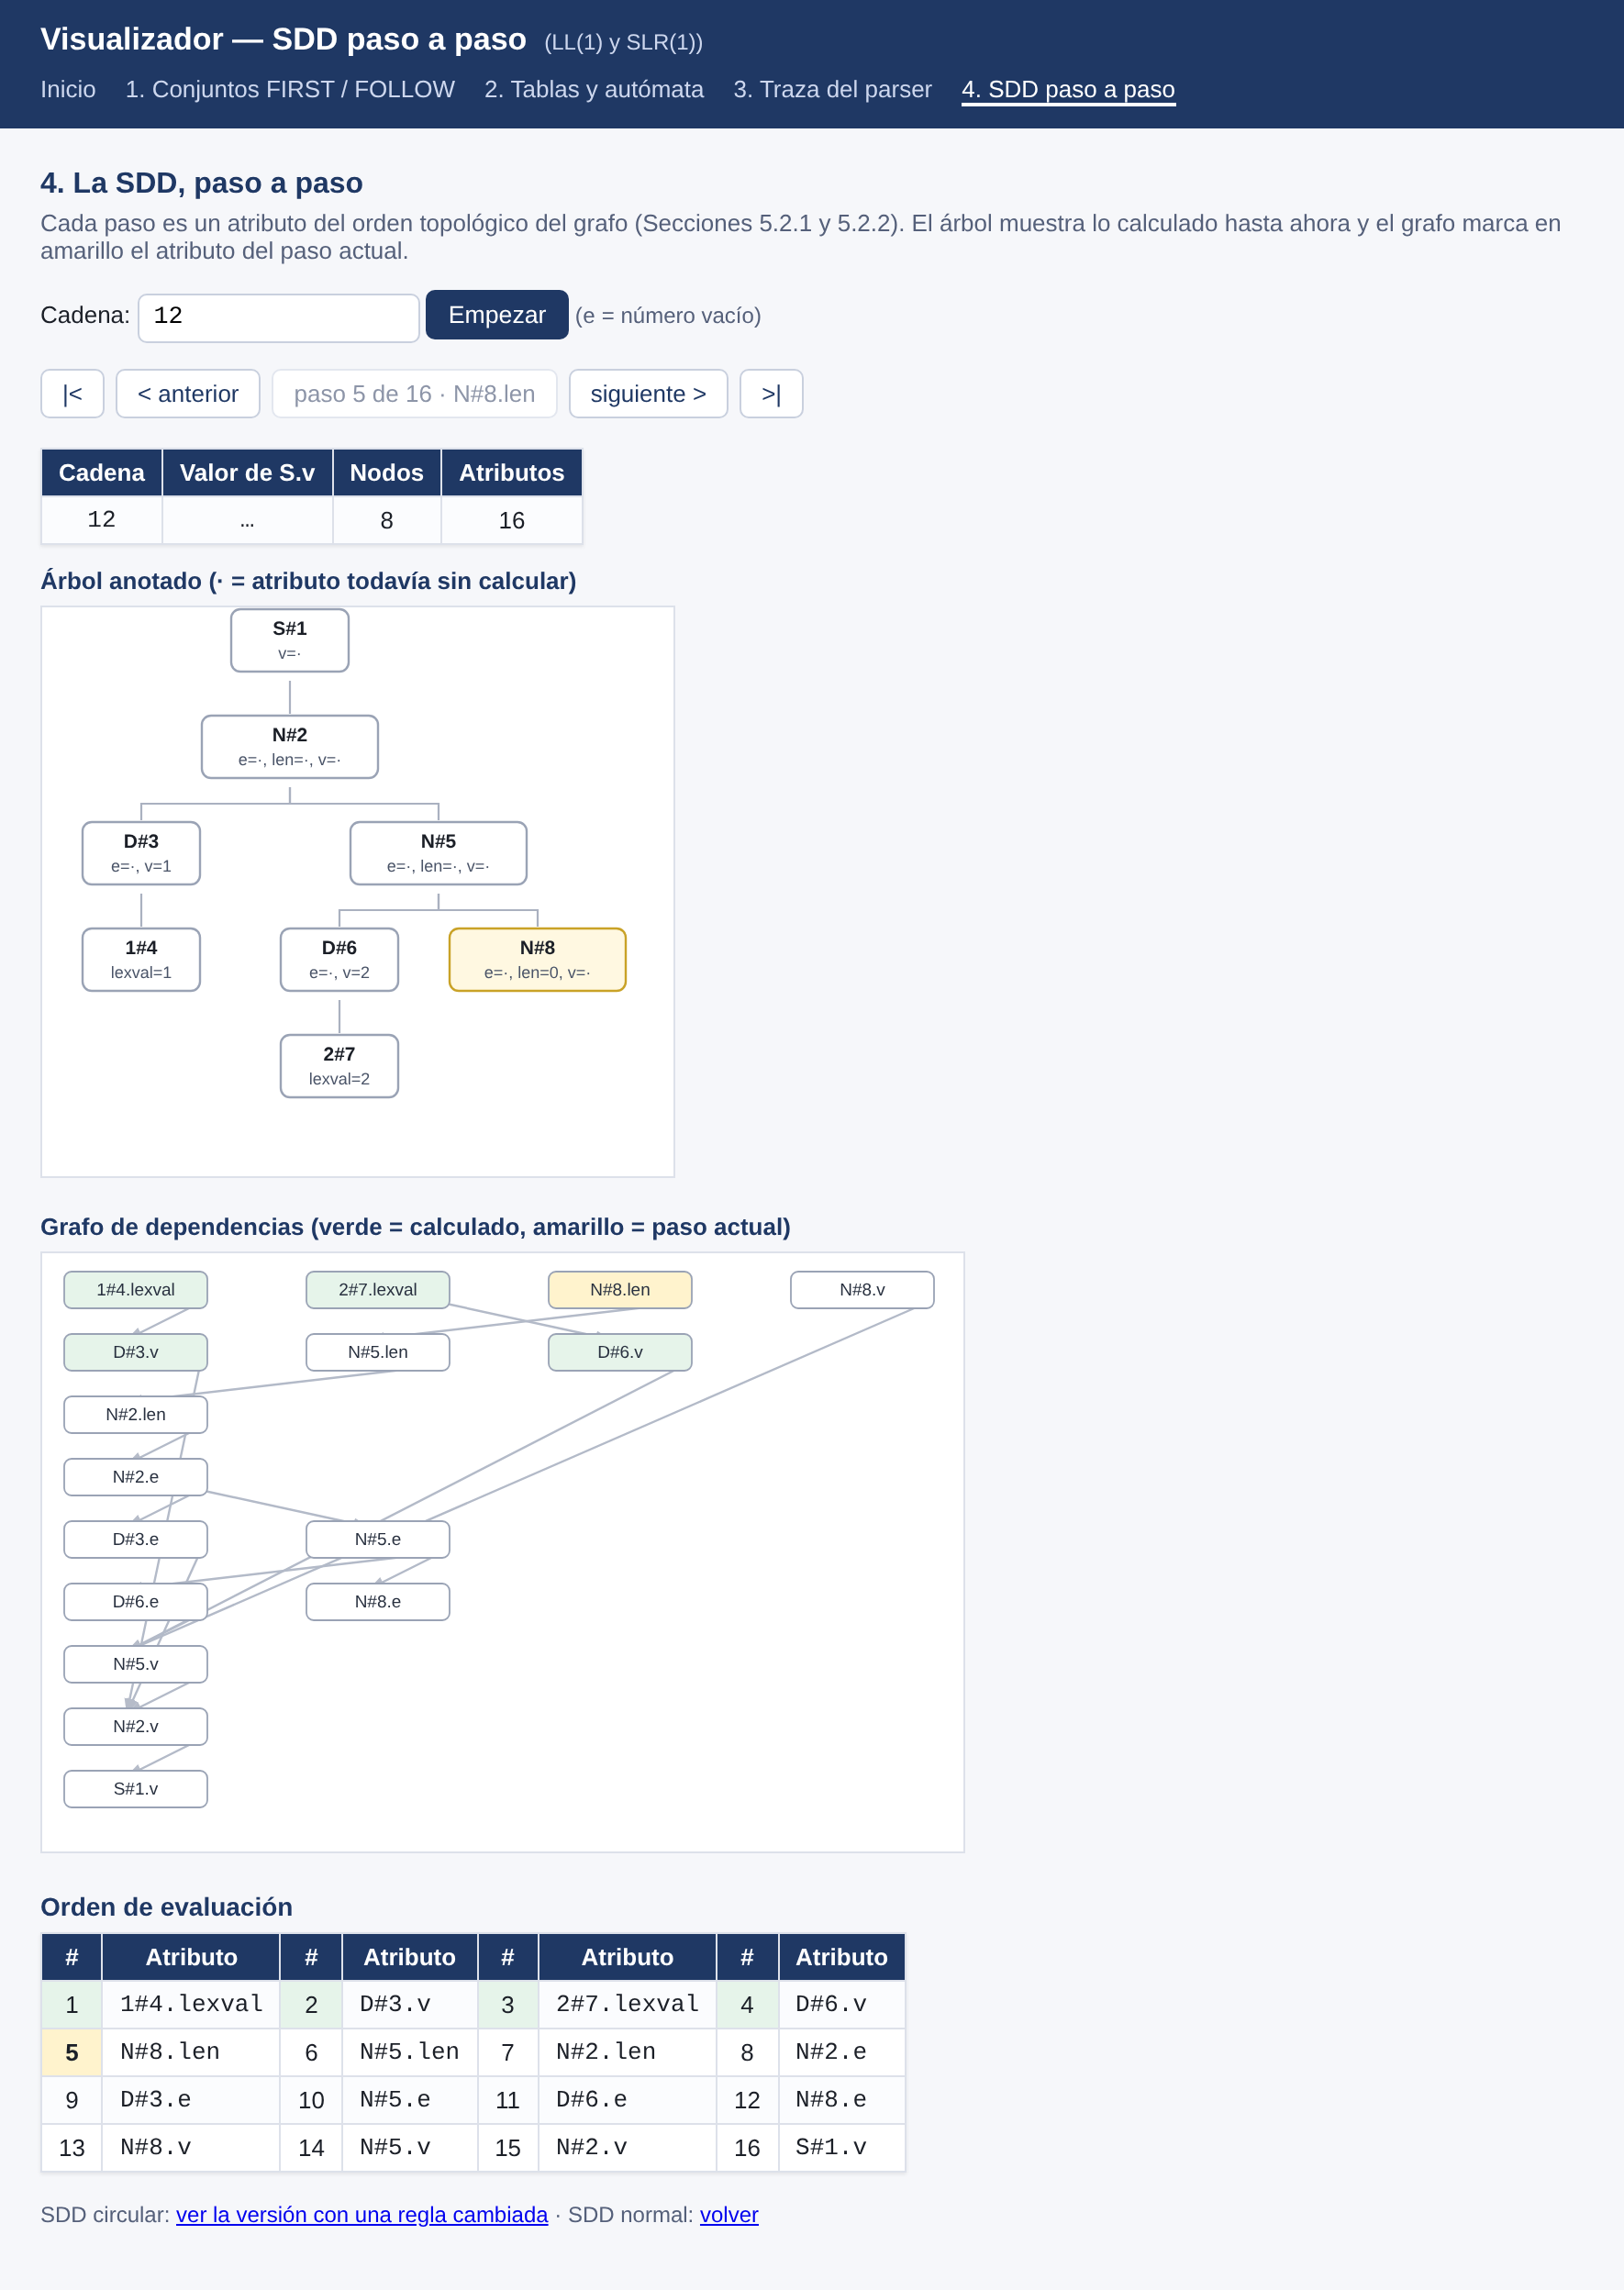
\includegraphics[width=5.75in]{figuras/visualizador.png}
\caption{The optional visualizer showing the evaluation of the SDD for the numeral \nt{12} at step 5
of 16: the tree with the attributes computed so far, the dependency graph with the same information
and the evaluation order at the bottom.}
\label{fig:visualizador}
\end{figure}

\subsection{Step 6: tests of the evaluator}

The five required strings were tested, including the shortest one (the empty numeral), a string with
repeated digits and one with leading zeros, plus a string that is not in the language and a numeral
of 300 digits to exercise deep nesting (the grammar is right recursive, so the tree is 300 levels
deep and the iterative traversals matter here). Table~\ref{tab:pruebas} summarises the runs.

\begin{table}[H]
\centering
\small
\caption{Runs of the evaluator.}
\label{tab:pruebas}
\begin{tabular}{@{}l l r r r@{}}
\toprule
\textbf{Input} & \textbf{Parsed} & \textbf{Value of S.v} & \textbf{Nodes} & \textbf{Attributes}\\
\midrule
1207 & yes & 1207 & 14 & 28\\
5 & yes & 5 & 5 & 10\\
\nt{e} (empty) & yes & 0 & 2 & 4\\
99999 & yes & 99999 & 17 & 34\\
0042 & yes & 42 & 14 & 28\\
12x & no & --- & --- & ---\\
\bottomrule
\end{tabular}
\end{table}

The 300-digit numeral gives the correct value (the test suite compares it against
\nt{int(cadena)}) and the program does not run out of recursion.

\paragraph{Circularity.} To show that the evaluator detects circular definitions, one rule of the
SDD is changed: in $S \to N$, instead of $N.e = N.len - 1$ the rule becomes $N.e = N.v$ (option
\nt{-{}-circular}). The exponent of the first digit then depends on the value of the number, which
depends on that same exponent: a cycle. With the string \nt{101} the program prints

\begin{lstlisting}[style=consola]
$ printf '101\n' | cat docs/gramatica_sdd.txt - | python3 main.py --sdd --circular
SDD is circular: N#2.v -> D#3.e -> N#2.e -> N#2.v
\end{lstlisting}

and stops without printing a tree: the cycle is $N.v \to D.e \to N.e \to N.v$, which is exactly the
loop of the modified rule against the value rule of the same production. The test suite asserts
this output and also asserts that nothing is evaluated when the graph is cyclic.

\section{Problems found and how we solved them}

\paragraph{Repeated alternatives created false conflicts.} A grammar is a \emph{set} of
productions, but the first version appended every alternative read from the input. With $S \to a\,a$
the same body received two different indices, the predictive table put two productions in
$M[S,a]$ and the SLR table produced a reduce/reduce conflict between two copies of the same
production. The fix is four lines in \nt{grammar.py} (store a body only if it is not already in the
list) and it corrected both parsers at once.

\paragraph{The reduction of $\varepsilon$ popped the whole stack.} In the LR parser, a reduction
$A \to \varepsilon$ must pop zero states. Written as \nt{del stack[-len(body):]} it pops the entire
stack, because \nt{-len(body)} is \nt{-0} and \nt{stack[-0:]} is the whole list in Python. There is
now an explicit branch for \nt{len(body) == 0}; the same trap appears in the tree construction,
where the node with no children must hang zero children and not all of them.

\paragraph{The alternatives of the input are separated by blanks, not the symbols.} Section 2.2 says
that an alternative is a sequence of symbols \emph{without} blanks, so $S \to aSb\ e$ has two bodies
and $S \to aS\ b\ e$ has three. Our first example in the README was written the wrong way: it
declared two nonterminals but only the nonterminal \nt{S}, and the alternatives were split in the
middle of a body. The test suite now fixes the format with an explicit test, so the mistake cannot
come back, and the README example is \nt{1} / $S \to aSb\ e$.

\paragraph{The numbering of the states changed between executions.} The item sets are
\nt{frozenset}, and iterating a set of tuples of strings depends on hash randomisation: the states
of the automaton were created in a different order in each execution, so the automaton printed in
this report would not match the one the program builds. The transitions are now traversed with
\nt{sorted()}, and the numbering is stable and reproducible. For the same reason, the vertices of
the dependency graph use the preorder number of the node instead of its memory address, which made
the evaluation order change from one run to the next.

\paragraph{The SDD wrote a value in the wrong node.} The rule $D.e = N.e$ belongs to the production
$N \to D\,N$ but defines an attribute of the child $D$, not of $N$. The first evaluator stored every
value in the node that owned the rule, so $D.e$ landed on $N$ and the next attribute that needed it
failed. The evaluator now stores the value in the node of the vertex (the symbol the position refers
to). This is a good example of why the SDD is described with positions: the position of the
attribute being defined is not always 0.

\paragraph{Recursion over the tree and over the string.} The natural way to write the tree traversals
is recursion, and with a 300-digit numeral the tree is 300 levels deep: Python's limit is 1000 and
the parser recursions add up. Every traversal (numbering, printing, dependency graph, cycle search)
uses an explicit stack, and the parsers use the stack of the book, so the depth of the tree is not
a limit.

\paragraph{Two details of the book.} The first is an erratum: step 1 of Algorithm 4.31 (p.~224) is
printed as adding the production to $M[A,a]$ for every $a$ in FIRST($A$), but the correct set is
FIRST($\alpha$), the FIRST of the body, as Example~4.32 shows; our table uses
\nt{first\_de\_cadena(cuerpo, first)}, which is the correct version. The second is in Algorithm 4.34
(Fig.~4.20, pp.~226--227): its loop ends when the top of the stack is \nt{\$} and never looks at the
input again, so it would accept \nt{aa} with the grammar $S \to a$. Our parser accepts only when the
stack is \nt{\$} \emph{and} the current input symbol is \nt{\$}, and the test suite fixes that case
(\nt{accept exige entrada en \$}) so the behaviour cannot regress.

\section{Conclusions}

The three items are implemented from the algorithms of the book, without transformations of the
input grammar and without external libraries, and they agree with each other: the same grammar that
FIRST/FOLLOW analyses is the one the two parsers accept, the two parsers build the same tree, and the
SDD is evaluated on that tree. The SDD of Item 3 is L-attributed but not S-attributed; one of its
inherited attributes depends on a synthesized attribute of the same symbol, so it cannot be evaluated
in a single pass with a fixed order, and we implemented the general dependency-graph method (which the
assignment requires in any case). The evaluator also
the evaluator detects circular definitions and reports the cycle instead of looping. The 93 tests of
the suite compare exact output, so a change in the format, in the tables or in the evaluation order
is caught immediately.

\begin{thebibliography}{9}
\bibitem{aho} Aho, A. V., Lam, M. S., Sethi, R., Ullman, J. D. \emph{Compilers: Principles,
Techniques, and Tools}, 2nd edition. Addison-Wesley, 2006. Sections 4.4, 4.5, 4.6, 5.1 and 5.2.
\bibitem{enunciado} Course assignment statement, SI2002 / ST0270 / CM0081 Formal Languages,
October 2026 (file \nt{docs/ENUNCIADO.md}).
\end{thebibliography}

\end{document}
